\subsection{Candidate Technologies}
Traditionally, edge devices were isolated cluster heads mainly forwarding traffic from their slaves to the cloud. Today, they are an integral part of the data flow pre-processing data and executing part of the business logic. The software running on these devices needs to be managed and with the increased number of device it is clear that the solution has to be centralized and efficient. There are  chapter will compare four different approaches on how to do this: local management, centralized management. \\
First,
% https://scholar.google.com/scholar?cluster=13680069378267225814&hl=de&as_sdt=0,5

\subsection{IoT Gateway Solutions}
https://www.bosch-iot-suite.com/service/gateway-software/
IoT gateway solutions include all technologies which do not involve orchestration based on containers. I will diferentiate between two categories, solutions based on orchestration and non-orchestrated solutions. The latter are solutions which are usually installed by an OEM and hard to update and maintain as they are not managed by a central entity. Orchestrated solutions on the other hand offer a central configuration point. These solutions were specifically developed for a distributed and large scale IoT environemnt. In many ways they are comparable to the solutions described in the next two subchapters. One example for such a solution is the Bosch IoT Gateway Software \cite{BoschIoT13:online}.

\begin{figure}[h!]
    \centering
    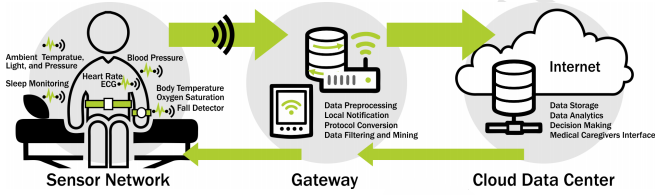
\includegraphics[scale=1.8]{figures/iotSetup.png}
    \caption{From the official Bosch documentation \cite{BoschIoT13:online}.}
    \label{fig:boschIoTGatewaySetup}
\end{figure}





\subsection{Disconnected Orchestrated Solutions}
IoT cluster solutions\\
Isolated k8s cluster: Solution k3s\\
Kubernetes cluster where edge is part of the cloud: kubeedge\\
% https://github.com/kubernetes/website/pull/13158



\subsection{Connected orchestrated solutions}
Edged: an agent that runs on edge nodes and manages containerized applications.
EdgeHub: a web socket client responsible for interacting with Cloud Service for the edge computing (like Edge Controller as in the KubeEdge Architecture). This includes syncing cloud-side resource updates to the edge, and reporting edge-side host and device status changes to the cloud.
CloudHub: a web socket server responsible for watching changes at the cloud side, caching and sending messages to EdgeHub.
EdgeController: an extended kubernetes controller which manages edge nodes and pods metadata so that the data can be targeted to a specific edge node.
EventBus: a MQTT client to interact with MQTT servers (mosquitto), offering publish and subscribe capabilities to other components.
ServiceBus: a HTTP client to interact with HTTP servers (REST), offering HTTP client capabilities to components of cloud to reach HTTP servers running at edge.
DeviceTwin: responsible for storing device status and syncing device status to the cloud. It also provides query interfaces for applications.
MetaManager: the message processor between edged and edgehub. It is also responsible for storing/retrieving metadata to/from a lightweight database (SQLite).

https://randomnerdtutorials.com/esp32-over-the-air-ota-programming/